\section{Proposed Relationship Prediction Approach}

Given a DHIN graph $G=(V,E)$, we decompose $G$ into a sequence of $t$ HIN graphs ${G_1, .., G_t}$ based on links with associated timestamps and then predict relationships in $G_{t+1}$. As mentioned in Definition \ref{problemdef}, we intend to predict existence of a given type of relationship (target meta path) between two given nodes. Thus we define a new type of graph, called \textit{augmented reduced graph}, that is generated according to a given heterogeneous network and a target relation meta path. 

%\begin{definition}[Augmented reduced graph]\label{def:ARG}
%Given a HIN graph $G=(V,E)$ and a target meta path $\mathcal{P}(A_i,A_j)$ between nodes of type $A_i$ and $A_j$, an \textit{augmented reduced graph} $G^\mathcal{P}=(V^\mathcal{P},E^\mathcal{P})$ is a weighted graph, where $V^\mathcal{P} \subseteq V$ and nodes in $V^\mathcal{P}$ are of type $A_i$ and $A_j$, edges in $E^\mathcal{P}$ indicates relationships of type $\mathcal{P}$ in $G$, and each edge $e^\mathcal{P} = (u, v, w)$ is a weighted edge from a vertex $u$ to a vertex $v$ with a weight $w=Sim(u,v)$ indicating a similarity measure between $u$ and $v$. $\Box$
%\end{definition}

\begin{definition}[\textbf{Augmented reduced graph}]\label{def:ARG}
Given a HIN graph $G=(V,E)$ and a target meta path $\mathcal{P}(A_i,A_j)$ between nodes of type $A_i$ and $A_j$, an \textit{augmented reduced graph} $G^\mathcal{P}=(V^\mathcal{P},E^\mathcal{P})$ is a graph, where $V^\mathcal{P} \subseteq V$ and nodes in $V^\mathcal{P}$ are of type $A_i$ and $A_j$, and edges in $E^\mathcal{P}$ indicate relationships of type $\mathcal{P}$ in $G$. $\Box$
\end{definition}


For example, an augmented reduced graph for the network in Figure \ref{sampleNetwork} and target meta path $\mathcal{P}(A,A)$=\textit{A--P--V--P--A} is a graph shown in Figure \ref{arg} whose nodes are of type \textit{Author} and whose edges represent \textit{publishing in the same venue}. %For example (\textit{Max}, \textit{Ada}) is an edge in the corresponding augmented reduced graph because they both published at KDD and ICDM. If we consider meta path $\mathcal{P}(A,A)$=\textit{A--P--A}, the augmented reduced graph represents a co-authorship graph, where nodes are of type \textit{Author} and edges, such as (\textit{Max}, \textit{Tom}), represent \textit{co-authorship}.


%\amin{modelling as bipartite graph}

\subsection{Homogenized Link Prediction}\label{def:HLP}

Once the given DHIN graph $G=(V,E)$ is decomposed to $t$ HIN graphs $G_1, .., G_t$, one solution to the relationship prediction problem (Definition \ref{problemdef}) is to build an augmented reduced graph $G_i^\mathcal{P}$ for each $G_i$ with respect to the given target meta path $\mathcal{P}$ and then predict a link in $G_i^\mathcal{P}$ instead of a path in $G_i$. In other words, we generate a homogenized version of a graph snapshot and apply a link prediction method. Figure \ref{targetARG} shows examples of such graphs at different time intervals. The intuition behind considering different snapshots, i.e., a dynamic network, rather than a single snapshot for link prediction is that we can incorporate network evolution patterns to increase prediction accuracy. Our hypothesis is that the estimated graph $\hat{G}_{i+1}^\mathcal{P}$ dependents on $\hat{G}_i^\mathcal{P}$. 

\begin{figure}[t]
\centering
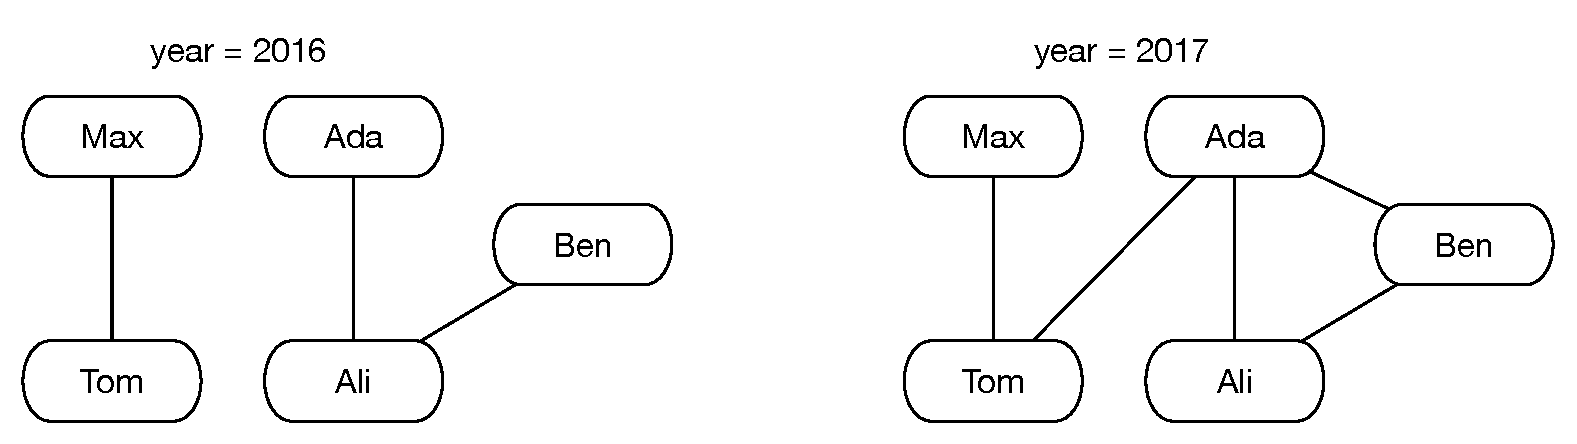
\includegraphics[trim = 0mm 5mm 0mm 0mm,width=0.85\textwidth]{figs/exampletargetARG.pdf}
\caption{Augmented reduced graphs for the network in Figure \ref{sampleNetwork} with respect to the target meta path \textit{A--P--A} (co-authorship) in 2016 and 2017.}\label{targetARG}
\end{figure}




Recently researchers have focused on inferring latent space of networks for link prediction \cite{Zhu2016,ye2013predicting,qi2013link,dunlavy2011temporal,menon2011link} based on the assumption that the probability of a link between two nodes depends on their positions in their latent space. Each dimension of the latent space characterizes an attribute, and the more two nodes share such attributes the more likely they connect (also known as homophily). Amongst such graph embedding methods, a few  \cite{dunlavy2011temporal,Zhu2016} considered dynamic networks. Inspired by %the matrix factorization approach presented by 
Zhu et al. \cite{Zhu2016}%for temporal link prediction in homogeneous networks
, we formulate our problem as follows: Given a sequence of augmented reduced graphs $G^\mathcal{P}_1, .., G^\mathcal{P}_t,$ we aim to infer a low rank $k$-dimensional latent space matrix $Z_i$ for each adjacency matrix $G^\mathcal{P}_i$ at time $i$ by minimizing 
%\begin{equation}\label{latentOrigEqu}
%    \begin{array}{l}
%\argmin\limits_{Z_1, .., Z_t}\sum\limits_{i=1}^{t}\left( \| G^\mathcal{P}_i-Z_{i}Z_{i}^T \right \|^2_F+\lambda \sum\limits_{i=1}^{t}\sum\limits_{v \in V^\mathcal{P}}(1-Z_{i}(v)Z_{i-1}(v)^T) 
%\\
%\text{subject to :} \forall v \in V^\mathcal{P},i,Z_{i}\geq 0, Z_{i}(v)Z_{i}(v)^T=1
%    \end{array}
%\end{equation}
\begin{equation}\label{latentOrigEqu}
    \begin{array}{l}
\argmin\limits_{Z_1, .., Z_t}\sum\limits_{i=1}^{t}\left(\left \| G^\mathcal{P}_i-Z_{i}Z_{i}^T \right \|^2_F+\lambda \sum\limits_{x \in V^\mathcal{P}}(1-Z_{i}(x)Z_{i-1}(x)^T) \right)
\\
\text{subject to :} \forall x \in V^\mathcal{P},i,Z_{i}\geq 0, Z_{i}(x)Z_{i}(x)^T=1
    \end{array}
\end{equation}
where $Z_i(x)$ is a temporal latent vector for node $x$ at time $i$, %$Z_i(x,j)$ indicates the position of $x$ in the $j^{th}$ dimension, 
$\lambda$ is a regularization parameter, and $1-Z_{i}(x)Z_{i-1}(x)^T$ penalizes sudden changes for $x$ in the latent space. This optimization problem can be solved using gradient descent. The intuition behind the above formulation is two fold: (1) node with similar latent space representation are more likely to connect with each other, and (2) nodes typically evolve slowly over time and abrupt changes in their connection network are less likely to happen \cite{zhang2014inferring}. 
% is that nodes with similar latent space representations are more likely to connect, and also nodes move smoothly in the latent space over time and it is less likely to have abrupt moves \cite{zhang2014inferring}. 
The matrix $G^\mathcal{P}_{t+1}$ can be estimated by $\Phi(f(Z_1,...Z_t))$, where $\Phi$ and $f$ are link and temporal functions, or simply by $Z_tZ_t^T$. Note that $Z_i$ depends on $Z_{i-1}$ as used in the temporal regularization term in Equation (\ref{latentOrigEqu}).

 
%To predict adjacency matrix $G^\mathcal{P}_{t+1}$, they used $Z_tZ_t^T$, however, they mentioned that $G_{t+1}$ can be formulated as $\Phi(f(Z_1,...Z_t))$, where $\Phi$ and $f$ are link and temporal functions that one may apply techniques such as nonparametric approaches \cite{Sarkar:2012} to learn them.

%can be solved for instance by using block-coordinate gradient descent \cite{Zhu2016}


\begin{algorithm}[t]
\caption{Homogenized Link Prediction}\label{alg1}
\begin{algorithmic}[1]\scriptsize
\REQUIRE A DHIN graph $G$, the number of snapshots $t$, a target meta path $\mathcal{P}(A,B)$, the latent space dimension $k$, the link to predict $(a,b)$ at $t+1$
%\ENSURE The predicted graph $G^\mathcal{P}$ at time $t+1$ based on the target relation $\mathcal{P}$
\ENSURE The probability of existence of link $(a,b)$ in $G^\mathcal{P}_{t+1}$

\STATE $\{G_1, .., G_t\} \leftarrow DecomposeGraph(G, t)$

\FOR {each graph $G_i=(V_i,E_i)$}
    %\STATE $G^R_i \leftarrow AugmentedReducedGraph(G_i,P,S)$
    %\STATE Let $a$ and $b$ be the node types of beginning and end of $\mathcal{P}$
    
    %\FOR {each path $p$ between nodes of type $a$ and $b$ in $S$}
    \FOR {each node $x \in V_i$ that $\phi(x)=A$}%of type $a$}
        \STATE Follow $\mathcal{P}$ to reach a node $y\in V_i$ that $\phi(y)=B$%of type $b$ 
        \STATE Add nodes x and y, and edge $(x,y)$ to the augmented reduced graph $G_i^\mathcal{P}$ 
\ENDFOR

\ENDFOR

\STATE $\{Z_1, .., Z_t\} \leftarrow MatrixFactorization(G^\mathcal{P}_1, .., G^\mathcal{P}_t, k)$

\STATE Return $Pr((a,b)\in E^\mathcal{P}_{t+1}) \leftarrow \sum_{i=1}^{k} Z_t(a,i)Z_t(b,i)$


%\STATE $G^\mathcal{P}_{t+1} \leftarrow Z_tZ^T_t$ 
%\STATE Return $G^\mathcal{P}_{t+1}$
\end{algorithmic}
\end{algorithm}




Algorithm \ref{alg1}  presents a concrete incorporation of Equation 1 for relation prediction. It takes as input a DHIN graph $G$, the number of graph snapshots $t$, a target relation meta path $\mathcal{P}(A,B)$, the latent space dimension $k$, and the link to predict $(a,b)$ at $t+1$. It first decomposes $G$ into a sequence of $t$ graphs $G_1, .., G_t$ by considering the associated timestamps on edges (line 1). Next from each graph $G_i$, a corresponding augmented reduced graph $G^\mathcal{P}_i$ is generated (lines 2-7) for which nodes are of type $a$ and $b$ (beginning and end of target  meta path $\mathcal{P}$). For example given $\mathcal{P}(A,A)$=\textit{A--P--A}, each $G^\mathcal{P}_i$ represents the co-authorship graph at time $i$. Finally by optimizing Equation (\ref{latentOrigEqu}) it infers latent spaces $Z_1, ...,Z_t$ (line 8) and estimates $G^\mathcal{P}_{t+1}$ using $Z_tZ_t^T$ (line 9). 




%\subsection{Meta path-based relationship prediction}
\subsection{Dynamic Meta Path-based Relationship Prediction}

The above homogenized approach does not consider different semantics of meta paths between the source and destination nodes and assumes that the probability of a link between nodes depends only on their latent features. For instance, as depicted in Figure \ref{targetARG}, \textit{Tom} and \textit{Ada} became co-authors in 2017 that can be due to publishing at the same venue in 2016, i.e., having two paths between them that passes through \textit{SIGIR}, as shown in Figure 2. Similarly \textit{Ben} and \textit{Ada} who published with a same author, \textit{Ali} in 2016, became co-authors in 2017. 
%On the other hand, Sun et al. \cite{sun2011ASONAM} proposed a supervised learning framework, called \textit{PathPredict}, that uses meta path-based features in a past time interval to predict the relationship building in a future time interval. It learns coefficients associated with features by maximizing the likelihood of new relationship formation. However, their model is learned based on one past interval and does not consider temporal changes as in \cite{Zhu2016}. 
%Our intuition is that leveraging meta path-based features along with latent space features can help to boost prediction accuracy. To this end, we combine latent features with meta path-based features in our model as described in Algorithm 2.
%Our hypothesis is that combining latent with topological features can increase prediction accuracy as we can learn latent features that fit the residual of meta path-based features. One way to combine these features is to incorporate meta path measures in Equation (\ref{latentOrigEqu}) by changing the loss function and regularization term as

We would like to further hypothesize that combining latent and topological features can increase prediction accuracy as we can learn latent features that fit the residual of meta path-based features. One way to combine these features is to incorporate meta path measures in Equation (\ref{latentOrigEqu}) by changing the loss function and regularization term as:
\begin{equation}\label{latentMetaEqu}
    \begin{array}{l}
\argmin\limits_{\boldsymbol{\theta_i},Z_i}\sum\limits_{i=1}^{t}\left \| G^\mathcal{P}_i - (Z_{i}Z_{i}^T + \sum\limits_{i=1}^{n}\theta_{i_{i-1}} \mathcal{F}^{\mathcal{P}_i}_{i-1}) \right \|^2_F+
\\ 
\lambda \sum\limits_{i=1}^{t}\left(\sum\limits_{x \in V^\mathcal{P}}(1-Z_{i}(x)Z_{i-1}(x)^T) + \sum\limits_{i=1}^{n} \theta_{i_i}^2\right)\\
    \end{array}
\end{equation}
where $n$ is the number of meta path-based features, $\mathcal{F}^{\mathcal{P}_i}$ is the $i^{th}$ meta path-based feature matrix defined on $G_i$, and $\theta_i$ is the weight for feature $f_i$. Although we can use a fast block-coordinate gradient descent \cite{Zhu2016} to infer $Z_i$s, it cannot be efficiently applied to the above changed loss function. This is because it requires computing meta paths for all possible pairs of nodes in $\mathcal{F}^{\mathcal{P}_i}$ for all snapshots, which is not scalable, as calculating similarity measures, such as Path Count or PathSim, can be very costly. For example computing path counts for \textit{A--P--V--P--A} meta path can be done by multiply adjacency matrices $AP\times PV\times VP\times PA$. 


%Thus we restrict it only to those links that make new connections in the next time interval or negative samples and use logistic regression.
As an alternative solution, we build a predictive model that considers a linear combination of topological and latent features. These features, however, can be interpolated in different ways that is beyond the scope of this work. Given the training pairs of nodes and their corresponding meta path-based and latent features, we apply logistic regression to learn the weights associated with these features. We define the probability of forming a \textit{new link} in time $t+1$ from node $a$ to $b$ as %$Pr(label=1|a, b; \boldsymbol{\theta}) = \frac{1}{e^{-z}+1}$, where $z=\sum\limits_{i=1}^{n}\theta_i.f_i(a,b)$ 
 $Pr(label=1|a, b; \boldsymbol{\theta}) = \frac{1}{e^{-z}+1}$, where $z=\sum\limits_{i=1}^{n}\theta_i f_t^{\mathcal{P}_i}(a,b) + \sum\limits_{j=1}^{k} \theta_{n+j}Z_t(a,j)Z_t(b,j)$, and $\theta_1,\theta_2,..., \theta_n$ and $\theta_{n+1},\theta_{n+2},..., \theta_{n+k}$ are associated weights for meta path-based features and latent features at time $t$ between $a$ and $b$. Given a training dataset with $l$ instance-label pairs, we use logistic regression with $L_2$ regularization to estimate the optimal $\boldsymbol{\theta}$ as:%where $\lambda \sum_{j=1}^{n+k} \theta_j^2$ is the regularization term, and $C>0$ is a penalty parameter. 

%$\boldsymbol{\hat{\theta}} = 
%\operatorname*{arg\,max}_{\boldsymbol{\theta}}\sum_i log Pr(y_i = 1|a_i, b_i; \boldsymbol{\theta}) - \alpha \sum_{j=1}^N \theta_j^2
%$

\begin{equation}
\boldsymbol{\hat{\theta}} = 
\argmin\limits_{\boldsymbol{\theta}}\sum_{i=1}^l -log Pr(label |a_i, b_i; \boldsymbol{\theta}) + \lambda \sum_{j=1}^{n+k} \theta_j^2
\end{equation}
 
We preferred to combine features in this learning framework since $G_i$ is very sparse and thus the number of newly formed links are much less compared to all possible links. Consequently calculating meta path-based features for the training dataset is scalable compared to the matrix factorization technique. Moreover, similar to \cite{sun2011ASONAM}, in order to avoid excessive computation of meta path-based measures between nodes that might not be related, we confine samples to pairs that are located in a nearby neighborhood. More specifically, for each source node $x$ in $G^\mathcal{P}_{i}$, we choose target nodes that are within two hops of $x$ but not in 1-hop, i.e, are not connected to $x$ in $G^\mathcal{P}_{i}$. We first find all target nodes that make a new relationship with $x$  in $G^\mathcal{P}_{i+1}$ and label respective samples as positive. Next we sample an equal number of negative pairs, i.e., those targets that do not make new connection, in order to balance our training set. Once the dataset is built, we perform logistic regression to learn the model and then apply the predictive model to the feature vector for the target link. The output probability can be later interpreted as a binary value based on a cut-off threshold.



%In the testing phase, we predict a data point $x$ as positive if $\theta^Tx > 0$, and negative otherwise.

%We derive \textbf{$\hat{\theta}$} which which maximizes the likelihood of all the training pairs.

%\cite{Zhu2016} approximated $G_{ij}$ with $\sum_{l=1}^{k} Z_{il}Z_{jl}$ and \cite{sun2011pathsim} with $\sum_{l=1}^{n} \theta_l f_l(i,j)$
%- $G_{ij} \approx  \sum_{l=1}^{n} \theta_l f_l(i,j) + \sum_{l=1}^{k} \beta_l Z_{il}Z_{jl}$
%$ \argmin\limits_{Z} \sum\limits_{(i,j)\in O} \left \| G_i(i,j) - \Phi(z_{i}^Tz_{j} + \theta^Tf_i(i,j)) \right \|^2_F $





\begin{algorithm}[t]
\caption{Dynamic Meta path-based Relationship Prediction}\label{alg2}
\begin{algorithmic}[1]\scriptsize
\REQUIRE A DHIN graph $G$, the number of snapshots $t$, a network schema $S$, a target meta path $\mathcal{P}(A,B)$, the maximum length of a meta path $l$, the latent space dimension $k$, the link to predict $(a,b)$ at $t+1$
%\ENSURE The predicted graph $G^\mathcal{P}$ at time $t+1$ based on the target relation $\mathcal{P}$
\ENSURE The probability of existence of link $(a,b)$ in $G^\mathcal{P}_{t+1}$

\STATE $\{G_1, .., G_t\} \leftarrow$ \textit{DecomposeGraph}$(G, t)$
%\STATE  $\{G^\mathcal{P}_1, .., G^\mathcal{P}_t\} \leftarrow BuildTargetAugmentedReducedGraph(G_1, .., G_t, \mathcal{P}(a,b))$
\STATE  Generate target augmented reduced graphs $G^\mathcal{P}_1, .., G^\mathcal{P}_t$ following Algorithm 1 lines 2-7

\STATE $\{\mathcal{P}_1, .., \mathcal{P}_n\} \leftarrow$ \textit{GenerateMetaPaths}$(S, \mathcal{P}(A,B), l)$

%\FOR {each graph $G_i=(V_i,E_i)$}
%
%    \FOR {each node $x \in V_i$ that $\phi(x)=A$}%of type $a$}
%	\FOR {each meta path $\mathcal{P}_j$}
%
%        \STATE Follow $\mathcal{P}_j$ to reach a node $y$ that $\phi(y)=B$%of type $b$}
%        \STATE $w_{xy} \leftarrow Similarity(x,y, G_i)$
%        \STATE Add nodes x and y, and edge $(x,y)$ with weight $w_{xy}$ to augmented reduced graph $G_i^{\mathcal{P}_j}$ 
%\ENDFOR
%\ENDFOR

%\STATE $\{Z_1, .., Z_t\} \leftarrow MatrixFactorization(G^{\mathcal{P}_j}_1, .., G^{\mathcal{P}_j}_t, k)$
%\STATE $G^{\mathcal{P}_j}_{t+1} \leftarrow Z_tZ^T_t$ 

%\ENDFOR

\STATE $\{Z_1, .., Z_t\} \leftarrow$ \textit{MatrixFactorization}$(G^\mathcal{P}_1, .., G^\mathcal{P}_t, k)$
%\STATE $\hat{G}^\mathcal{P}_{t} \leftarrow Z_{t-1}Z^T_{t-1}$ and  $\hat{G}^\mathcal{P}_{t+1} \leftarrow Z_tZ^T_t$


\FOR {each pair $(x,y)$, where $x\in V^\mathcal{P}_{t-1}$ and $y\in N(x)$ is a nearby neighbor of $x$ in $G^\mathcal{P}_{t-1}$}

\STATE Add feature vector $\langle$$f^{\mathcal{P}_i}_{t-1}(x,y)$ for $i=1..n$, $Z_{t-1}(x,j)Z_{t-1}(y,j)$ for $j=1..k)\rangle$ to the training set $T$ with \textit{label}=1 if $(x,y)$ is a new link in $E^\mathcal{P}_{t}$ otherwise \textit{label}=0.

%\STATE Add the feature vector $\langle$ $f^{\mathcal{P}_1}_{t-1}(x,y)$, $f^{\mathcal{P}_2}_{t-1}(x,y)$, ..., $f^{\mathcal{P}_n}_{t-1}(x,y)$, $\hat{G}^\mathcal{P}_{t}(x,y)\rangle$ to the training set $T$ with \textit{label}=1 if $(x,y)$ is a new link in $E^\mathcal{P}_{t}$ otherwise \textit{label}=0.

\ENDFOR

\STATE $model \leftarrow$ \textit{Train}$(T)$
%\STATE Return $Pr((a,b)\in E^\mathcal{P}_{t+1})$ $\leftarrow$ \textit{Test}($model$, $\langle$ $f^{\mathcal{P}_1}_{t}(a,b)$, $f^{\mathcal{P}_2}_{t}(a,b)$, ..., $f^{\mathcal{P}_n}_{t}(a,b)$, $\hat{G}^\mathcal{P}_{t+1}(a,b)\rangle)$

\STATE Return $Pr((a,b)\in E^\mathcal{P}_{t+1})$ $\leftarrow$ \textit{Test}($model$, $\langle$$f^{\mathcal{P}_i}_{t}(a,b)$ for $i=1..n$, $Z_t(a,j)Z_t(b,j)$ for $j=1..k)\rangle)$

\end{algorithmic}
\end{algorithm}


%Our intuition is that leveraging meta path-based features along with latent space features can help to boost prediction accuracy. To this end, we combine latent features with meta path-based features in our model as described in Algorithm 2.

We describe steps for building and applying our predictive model, called \textit{MetaDynaMix}, in Algorithm \ref{alg2}. The algorithm takes as input a DHIN graph $G$, the number of graph snapshots $t$, a network schema $S$, a target relation meta path $\mathcal{P}(A,B)$, the maximum length of a meta path $l$, the latent space dimension $k$, and the link to predict $(a,b)$ at $t+1$. Similar to Algorithm \ref{alg1}, it decomposes $G$ into a sequence of graphs (line 1). Next it generates augmented reduced graphs $G^\mathcal{P}_i$s from $G_i$s based on $\mathcal{P}$ for nodes which are of type $A$ and $B$ (beginning and end of meta path $\mathcal{P}$) (line 2) as explained in Algorithm 1. It then produces the set of all meta paths between nodes of type $A$ and type $B$ defined in $\mathcal{P}(A,B)$ (line 3). This is done by traversing the network schema $S$ (for instance through BFS traversal) and generating meta paths with the maximum length of $l$. It then applies matrix factorization to find latent space matrices $Z_i$ (line 4). %On this basis, it then calculates the estimated augmented reduced graph $\hat{G}^\mathcal{P}$ at times $t$ and $t+1$ (line 5). 
Next it creates a training dataset for sample pairs $(x,y)$ with feature set containing meta path-based measures $f^{\mathcal{P}_i}_t(x,y)$ for each meta path $\mathcal{P}_i$, and latent features $Z_t(a,j)Z_t(b,j)$ for $j=1..k$ at time $t$, and \textit{label}=1 if $(x,y)$ is a new link in $G^\mathcal{P}_{t+1}$ otherwise \textit{label}=0 (lines 5-7). Subsequently the algorithm trains the predictive model (line 8), generates features for the given pair $(a,b)$, and tests it using the trained model (line 9). %In the following section we explain our learning technique in detail.

% \begin{equation}\label{latentEqu}
%     \begin{array}{l}
% \argmin\limits_{Z_1, .., Z_t}\sum\limits_{i=1}^{t}\left \| G^{R_i}_i-Z_{i}Z_{i}^T \right \|^2_F+\lambda \sum\limits_{i=1}^{t}\sum\limits_{u}(1-Z_{i}(u)Z_{i-1}(u)^T) 
% \\
% \text{subject to :} \forall u,i,Z_{i}\geq 0, Z_{i}(u)Z_{i}(u)^T=1
%     \end{array}
% \end{equation}


%* Restrict pathSim to 3-hops and not beyond


%\begin{equation}\label{latentAndTopologicalEqu}
%    \begin{array}{l}
%\argmin\limits_{\boldsymbol{\theta},Z_1, .., Z_t}\sum\limits_{i=1}^{t}\left \| G_i - (Z_{i}Z_{i}^T + \sum\limits_{i=1}^{n}\theta_{i_i}\mathcal{F}_{i_i}) \right \|^2_F + \lambda (\sum\limits_{i=1}^{t}\sum\limits_{u}(1-Z_{i}(u)Z_{i-1}(u)^T)  + \sum\limits_{i=1}^{t} \sum\limits_{i=1}^{n} \theta_{i_i}^2)\\
%    \end{array}
%\end{equation}


%\subsubsection{The predictive model.}
%\subsubsection{Combining Latent and Meta Path-based Features.} => moved before Alg 2 description








% https://arxiv.org/pdf/1803.00744.pdf

%We perform leave-one-patient-out testing, where all data belonging to a single patient are left out in a particular test fold. All hyper-parameters were chosen through a nested cross-validation performed on the training data alone. We used the area under the ROC curve (AUROC) metric to evaluate our classifiers. We use the method presented by DeLong et al. [27] to compute 95\% confidence intervals and to perform statistical significance tests to compare competing prediction methods (significance level was set at 5\%). All reported p values are based on a two-sided z-test.

%[27] DeLong, E.R., DeLong, D.M., Clarke-Pearson, D.L.: Comparing the areas under two or more correlated receiver operating characteristic curves: a nonparametric approach. Biometrics (1988) 837?845




% \begin{algorithm}[h]
% \caption{Generate Predicted Graph}\label{alg1}
% \begin{algorithmic}[1]
% \REQUIRE A dynamic heterogeneous graph $G$, number of graph snapshots $t$, network schema $S$, target relation $R(a,b)$ between nodes of type $a$ and $b$, maximum length of a meta path $l$, latent space dimension $k$
% \ENSURE The predicted graph $G^R$ at time $t+1$ based on the given target relation $R$

% \STATE $\{G_1, .., G_t\} \leftarrow DecomposeGraph(G, t)$

% \STATE $\{\mathcal{P}_1, .., \mathcal{P}_n\} \leftarrow GenerateMetaPaths(S,R,l)$

% \FOR {each heterogeneous graph $G_i$}
%     %\STATE $G^R_i \leftarrow AugmentedReducedGraph(G_i,R,S)$
    
%     \FOR {each path $p$ between nodes of type $a$ and $b$ in $S$}
%     \FOR {each node $i$ of type $a$ in $G$}
%         \STATE follow $p$ to reach a node $j$ of type $b$ in $G$ 
%         \STATE $w_{ij} \leftarrow PathSim(i,j)$
%         \STATE add edge $(i,j)$ to graph $G^R$ with weight $w_{ij}$
%     \ENDFOR
% \ENDFOR

    
% \ENDFOR
% %\STATE $G^R_{t+1} \leftarrow matrix factorization(G^R,k)$ \cite{Zhu2016}
% \STATE Infer temporal latent spaces $Z_1, .., Z_t$ by optimizing Eq. \ref{latentEqu}

% \STATE $G^R_{t+1} \leftarrow Z_tZ^T_t$ 

% \STATE return $G^R_{t+1}$
% \end{algorithmic}
% \end{algorithm}


%The process of creating an augmented reduced graph is presented in Algorithm \ref{alg2}.

% \begin{algorithm}[h]
% \caption{Generate augmented reduced graph}\label{alg2}
% \begin{algorithmic}[1]
% \REQUIRE A heterogeneous graph $G$, target relation $R(a,b)$ between nodes of type $a$ and $b$, network schema $S$
% \ENSURE An augmented reduced graph $G^R$ based on the given target relation $R$

% \FOR {each path $p$ between nodes of type $a$ and $b$ in $S$}
%     \FOR {each node $i$ of type $a$ in $G$}
%         \STATE follow $p$ to reach a node $j$ of type $b$ in $G$ 
%         \STATE $w_{ij} \leftarrow PathSim(i,j)$
%         \STATE add edge $(i,j)$ to graph $G^R$ with weight $w_{ij}$
%     \ENDFOR
% \ENDFOR

% \STATE return $G^R$
% \end{algorithmic}
% \end{algorithm}